\documentclass{beamer}

\input{../../spec_files/course_preamble.tex}
\subtitle{Foundations of Neuro-Symbolic AI}
\date{Summer Term 2026}
\author[FONS]{Alex Goessmann}
\institute[]{
    University of Applied Science Würzburg-Schweinfurt
%    Weierstrass Institute for Applied Analysis and Stochastic
}

%\newcommand{\techwstitle}{
%\small
%%Workshop \\
%Logik für Erklärbare KI:
%Technische Einführung in das ENEXA Projekt}
%\newcommand{\smalltechwstitle}{ENEXA Workshop}

%\newcommand{\techwsdate}{15.+16. July, 2024}

%\newcommand{\techwsauthors}{
%Alex Goessmann
%}

%\newcommand{\techwsinclude}{
%	\usepackage{../../spec/beamercolorthemeclaw}
%	\usepackage{/Users/alexgoessmann/Documents/ENEXA/latex_macros/beamer_template/beamerfontthemeclaw}
%	\usepackage{/Users/alexgoessmann/Documents/ENEXA/latex_macros/beamer_template/beamerinnerthemeclaw}
%	\usepackage{/Users/alexgoessmann/Documents/ENEXA/latex_macros/beamer_template/beamerouterthemeclaw}
%
%	\input{/Users/alexgoessmann/Documents/ENEXA/latex_macros/packages.tex}
%	\input{/Users/alexgoessmann/Documents/ENEXA/latex_macros/macros.tex}
%	\input{/Users/alexgoessmann/Documents/ENEXA/latex_macros/macros_tc.tex}
%	\input{/Users/alexgoessmann/Documents/ENEXA/latex_macros/tikz_blocks.tex}
%
%	\subtitle{\techwstitle}
%	\date[\techwsdate]{\techwsdate}
%	\author[\smalltechwstitle]{\techwsauthors}
%	\institute[]{\eupic}
%}

\newcommand{\techwschapterone}{I-Tensors}
\newcommand{\techwschaptertwo}{II-Probabilities}
\newcommand{\techwschapterthree}{III-Logics}
\newcommand{\techwschapterfour}{IV-Applications}

\newcommand{\eupic}{
\begin{center}
	%\includegraphics[width=4cm]{/Users/alexgoessmann/Documents/ENEXA/latex_macros/images/fundedEU.png}
\end{center}
}

\newcommand{\enexadateveublock}{
\begin{center}\begin{tikzpicture}
  	%\node [anchor=center] at (0,0) {\includegraphics[width = 1.5cm]{/Users/alexgoessmann/Documents/ENEXA/latex_macros/images/DATEV.png}};
	%\node [anchor=center] at (2.5,0.5) {\includegraphics[width = 3.5cm]{/Users/alexgoessmann/Documents/ENEXA/latex_macros/images/enexa.png}};
	%\node [anchor=center] at (2.55,-0.5) {\includegraphics[width = 3cm]{/Users/alexgoessmann/Documents/ENEXA/latex_macros/images/fundedEU.png}};
\end{tikzpicture}\end{center}
}


%% OLD
\newcommand{\aselectionvariable}{L}
\newcommand{\vselectionvariable}{L}
\newcommand{\fselectionvariable}{L}
\newcommand{\cselectionvariable}{L}
\newcommand{\individualorder}{n}
\newcommand{\variableof}[1]{\indvariableof{#1}}
\newcommand{\sindex}{s}
\newcommand{\pindex}{p}
\newcommand{\oindex}{o}
\newcommand{\exquery}{q}
%\newcommand{\datapointof}[1]{x^{#1}}
\newcommand{\atomicqueryof}[1]{g_{#1}}
\newcommand{\facsystem}{\shortcatvariables}
\newcommand{\margprobof}[1]{\probat{#1}}
\newcommand{\mlnprobabilityof}[1]{\expdistof{#1}}
%\newcommand{\oldenexadateveublock}{
%	\begin{center}
%	\begin{minipage}{0.2\textwidth}
%		\begin{center}
%			\includegraphics[width = 2.5cm]{images/DATEV.png}
%		\end{center}
%	\end{minipage}
%	\begin{minipage}{0.55\textwidth}
%		\begin{center}
%			\includegraphics[width=5.5cm]{images/enexa.png} \\
%			\includegraphics[width=5.5cm]{images/fundedEU.png} \\
%		\end{center}
%	\end{minipage}
%	\end{center}
%}

\title[Neuro-Symbolic AI]{
	\techwschapterfour \\
	{\huge Neuro Symbolic AI}
}

\begin{document}



{\frame[plain]{\titlepage}}

\begin{frame}{Hochreiter: Towards a Broad AI}
 {\small Communications of the ACM, April 2022}

"Europe`s Opportunity for a Broad AI: \\
{ \it
The most promising approach to a broad AI is a neuro-symbolic AI, that is, a bilateral AI that combines methods from symbolic and sub-symbolic AI."}

\begin{center}
	\includegraphics[width=9cm]{./hochreiter_pic.png} 
\end{center}



\end{frame}

\begin{frame}{The Symbolic Paradigm}

\newcommand{\stanspace}{\hspace{0.5cm}\\}

\begin{minipage}{0.65\linewidth}
\begin{center} \it
How to represent knowledge? \\
$\rightarrow$ {\bf Logical Syntax} \\
\stanspace
How to interpret knowledge? \\
$\rightarrow$ {\bf Logical Semantics}
\end{center}
%Formal Logic:
%\begin{itemize}
%	\item Syntax: 
%	\item Semantics: 
%\end{itemize}
\end{minipage}
\begin{minipage}{0.25\linewidth}
\begin{center}
\includegraphics[width=2cm]{aristotle.png}\\
{\small Aristotle}
\end{center}
\end{minipage}

\begin{block}{Symbolic AI: Reasoning based on Logic}
	\begin{itemize}
		\item Data and models represented by logical syntax
		\item Learning and inference based on logical semantics
	\end{itemize}
	\textbf{Advantage:} Model explainability in its purest form (ante-hoc)
\end{block}

%Challenges:
%\begin{itemize}
%	\item Design of efficient algorithms
%	\item Incorporation of data and uncertainty 
%\end{itemize}

\end{frame}


\begin{frame}{The Neural Paradigm}

\begin{block}{Sub-symbolic AI: Computations in Neural Architectures}
	\begin{itemize}
		\item Expressivity of Deep Networks: Effective representation of Data
		\item Differentiable parametrization 
	\end{itemize}
	\textbf{Problem:} Black-box when not designed otherwise
\end{block}
\ \\
\medskip
Why deep and not shallow networks?
\begin{itemize}
	\item \emph{Physical explanations:} Deep neural networks appear naturally in use cases
	\item \emph{Mathematical explanations:} Deep neural networks have astonishing approximation properties
\end{itemize}
\end{frame}

\begin{frame}{Generation processes by deep layers}
	\begin{center}
 		\includegraphics[height=6cm]{generation.png}\\
		{\small Lin, Tegmark, Rolnick: Why does deep and cheap learning work so well? \\
		 Journal of Statistical Physics, 2017}
	\end{center}

\end{frame}


%\begin{frame}{}
%\end{frame}


\begin{frame}{Combining the paradigms: Hierarchical structure of Logical Formulas}

Logical formulas have an iterative decomposition structure into subformulas $\exformula_1,\exformula_2$ until they are at atomic level:
\begin{align}
	\exformula = \exformula_1 \exconnective \exformula_2
\end{align}

\textbf{Example:} Variables $a$ or $b$ implied by another variable $c$
 	\[ \exformula = \big( c \Rightarrow a \lor b \big)  = \big(a \lor b \lor \lnot c \big) \]
\begin{center}
	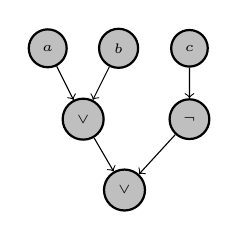
\begin{tikzpicture}[scale=0.3] % , baseline = -3.5pt



	\node [circle, draw, thick, fill=gray!50] (T1) at (0,0) {\tiny $a$};
	\node [circle, draw, thick, fill=gray!50] (T2) at (3,0) {\tiny $b$};
	\node [circle, draw, thick, fill=gray!50] (T3) at (6,0) {\tiny $c$};
	
	\node [circle, draw, thick, fill=gray!50] (and) at (1.5,-3) {\tiny $\lor$};
	\node [circle, draw, thick, fill=gray!50] (not) at (6,-3) {\tiny $\lnot$};	
	
	\draw [->] (T1) -- (and);
	\draw [->] (T2) -- (and);
	
	\draw [->] (T3) -- (not);	
	
	\node [circle, draw, thick, fill=gray!50] (head) at (3.25,-6) {\tiny $\lor$};
	
	\draw [->] (and) -- (head);
	\draw [->] (not) -- (head);			



\end{tikzpicture}
\end{center}

%\begin{block}{Towards Neuro-Symbolic AI}
%	The composability of logical formulas bears a neural architecture.
%	%Use this structure to define a neuro-symbolic architecture.
%\end{block}

\end{frame}




\begin{frame}{Challenge: Overparametrization by Logical Formulas}

A system with \emph{$\atomorder$ binary variables}
\begin{center}
	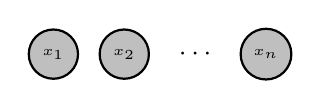
\begin{tikzpicture}[scale=0.3] % , baseline = -3.5pt


	\node [circle, draw, thick, fill=gray!50] (T1) at (0,0) {\tiny $x_1$};
	\node [circle, draw, thick, fill=gray!50] (T2) at (3,0) {\tiny $x_2$};

\node[anchor=center] (text) at (6,0) {$\cdots$};

	\node [circle, draw, thick, fill=gray!50] (T3) at (9,0) {\tiny $x_n$};
	

\end{tikzpicture}
\end{center}
has a number of states
	\[ \#\big\{x_1, \ldots, x_n \in \{0,1\} \big\} = 2^\atomorder \, .  \]
Whereas the \emph{number of logical formulas} is
	\[ 2^{\left(2^\atomorder\right)} \, . \]
For $\atomorder = 10$ binary variables we have
	\[2^{\left(2^{10}\right)} >10^{300} \, , \]
whereas the number of atoms in the known universe is $~10^{80}$.

\end{frame}




\begin{frame}{Learning Markov Logic Networks}
	
	\begin{block}{Two learning tasks}
		Given data we learn a Markov Logic Network by:
		\begin{itemize}
			\item \emph{Structure Learning}: Find the formulas $\exformula$ to be activated.
			\item \emph{Weight Estimation}: Find the optimal weights $\weightof{\exformula}$ to the formulas.
		\end{itemize}
	\end{block}
	
	While Weight Estimation is efficiently solvable, Structure Learning faces
	\begin{itemize}
		\item enormous search spaces: $2^{(2^\atomorder)}$ formulas to $\atomorder$ atoms
		\item computational demand to evaluate single formulas
	\end{itemize}
	
	%Learning means \emph{finding the active formulas}. \\
	\medskip
	We ease these problems by a tensor network decompositions of
	\begin{itemize}
		\item hypothesis formulas, by \emph{formula selecting neurons}
		\item log-likelihood losses and its gradients 
	\end{itemize}
	%\medskip
	%We construct Superposed Formula Tensors based on skeleton formulas and choice axis of components in them:
%	\begin{align}
%		\nonumber \mathcal{S} =& \exformula_1 \exconnective_2 \exformula_3 \quad \text{with candidate lists:} \\
%		\nonumber & \quad \exformula_1 : ["Atom1","Atom2","Atom3"] \\
%		\nonumber & \quad \exconnective_2 : ["and","or","implies"] \\ 
%		\nonumber & \quad \exformula_3 : ["Atom1","Atom2","Atom3"]
%	\end{align}
	%\medskip
	%When the formulas are known: \emph{Entropy Maximization} provides best weights.
\end{frame}




\begin{frame}{Structure Learning}

We take an ensemble perspective: 
\begin{itemize}
	\item Each formula has limited expressivity, thus we have to use collections
	\item We learn in a greedy way, that is choose best formula in each step
\end{itemize}

\begin{block}{Learning an additional formula to a given distribution}
	Given a hypothesis set $\formulaset$ and a current distribution $\probtensor$ we want to add the best formula $\exformulain$.
	We approach this by
	\begin{itemize}
		\item Finding an efficient representation of the formulas as a tensor network
		\item Contraction with the gradient of the likelihood 
		\item Search for the maximum likelihood ascent among the formulas
	\end{itemize}
%	From a set of $\seldim$ formulas $\{\exformula_{\selindex} : \selindexin\}$
\end{block}

\end{frame}



\begin{frame}{Representing multiple formulas}

\begin{block}{Trick: Selection Variables}
	Add argument to the formulas representing the selection choice among the hypothesis set $\formulaset$.
	Corresponding random variables are called \emph{selection variables} $\selinputvariable$. 
\end{block}

	Given a set of $\seldim$ formulas $\{\exformula_{\selindex} : \selindexin\}$, we define the formula selecting map as
		\[  \fselectionmap : \atomstates \times [\seldim] \rightarrow [2] \]
	defined for $\selindexin$ by
		\[ \fselectionmap(\atomindices,\selindex) =  \exformula_{\selindex}(\atomindices) \, . \]

\end{frame}


\begin{frame}{Representation as a Tensor Network}

Given a set of $\seldim$ formulas $\{\exformula_{\selindex} : \selindexin\}$, we define the formula selecting map as
	\[  \fselectionmap : \atomstates \times [\seldim] \rightarrow [2] \]
defined for $\selindexin$ by
	\[ \fselectionmap(\atomindices,\selindex) =  \exformula_{\selindex}(\atomindices) \, . \]
\medskip
We depict formula selecting maps by
\begin{tikzpicture}[scale=0.35, thick] % , baseline = -3.5pt

    \begin{scope}
        [shift={(-20,0)}]
        \node[anchor=center] (text) at (-1,3) {${a)}$};

        \node [circle, draw, thick, fill=\nodegrayscale, minimum size = \nodeminsize] (T1) at (0,0) {\colorlabelsize $\catvariableof{0}$};
        \node [circle, draw, thick, fill=\nodegrayscale, minimum size = \nodeminsize] (T2) at (3,0) {\colorlabelsize $\catvariableof{1}$};
        \node[anchor=center] (text) at (6,0) {${\cdots}$};
        \node [circle, draw, thick, fill=\nodegrayscale, minimum size = \nodeminsize] (T3) at (9,0) {};
        \node[anchor=center] (text) at (9,0) {\colorlabelsize $\catvariableof{\seldim\shortminus1}$};

        \node [circle, draw, thick, fill=\nodegrayscale, minimum size = \nodeminsize] (T4) at (12,3) {};
        \node[anchor=center] (text) at (12,3) {\colorlabelsize $\selvariable$};

        \draw[->-] (6,3) -- (6,6);

        \node [circle, draw, thick, fill=\nodegrayscale, minimum size = \nodeminsize] (S) at (6,6) {};
        \node[anchor=center] (text) at (6,6) {\colorlabelsize $\headvariableof{\fselectionmap}$};

        \draw[->-] (T1) -- (6,3);
        \draw[->-] (T2) -- (6,3);
        \draw[->-] (T3) -- (6,3);
        \draw[->-] (T4) -- (6,3);

    \end{scope}


    \node[anchor=center] (text) at (-1,3) {${b)}$};


    \begin{scope}
        [shift={(0,-2)}]
        \draw[-<-] (0,1)--(0,-1) node[midway,left] {\colorlabelsize $\catvariableof{0}$};
        \draw[-<-] (1.5,1)--(1.5,-1) node[midway,left] {\colorlabelsize $\catvariableof{1}$};
        \node[anchor=center] (text) at (3,0) {$\cdots$};
        \draw[-<-] (4,1)--(4,-1) node[midway,right] {\colorlabelsize $\catvariableof{\seldim\shortminus1}$};
    \end{scope}

    \draw (-1,1) rectangle (5,-1);
    \node[anchor=center] (text) at (2,0) {$\bsencodingof{\fselectionmap}$};
    \draw[->-] (2,1) -- (2,3) node[midway, right]  {\colorlabelsize $\headvariableof{\fselectionmap}$};
    \draw[-<-] (5,0) -- (7,0) node[midway, above] {\colorlabelsize $\selvariable$};


\end{tikzpicture}

\begin{itemize}
	\item[a)] Introduction of selection variables to the graphical model
	\item[b)] Tensor Core with selection variable stored in an incoming leg
\end{itemize}

\end{frame}


\begin{frame}{Design of Formula selecting maps}

We provide two building blocks by the
\begin{itemize}
	\item Choice of connections ($\sim$ support of the weights): \\ \emph{Variable selecting maps}
	\item Choice of activations ($\sim$ value of the weights): \\ \emph{Connective selecting maps}
\end{itemize}
and combine both in a
\begin{itemize}
	\item Symbolic neuron: Choice of a connective and variables passed into arguments
	\item Symbolic architecture: Collection of neurons with layerwise dependencies on each other
\end{itemize}


\end{frame}


\begin{frame}{Variable selecting maps}

\begin{definition}[Variable selecting map]
	Given a set of variables enumerated by $[\seldim]$, we call the map
	\begin{align}
		\vselectionmap:  \left(\bigtimes_{\selindex\in[\seldim]}[2]\right) \times [\seldim]  \rightarrow [2]
	\end{align}
	defined coordinatewise by
	\begin{align}
		\vselectionmap(\atomlegindexof{0},\ldots, \atomlegindexof{\seldim-1}, \selindex) = \atomlegindexof{\selindex}
	\end{align}
	the corresponding \emph{variable selecting map}.
\end{definition}
	

\end{frame}


\begin{frame}{Tensor Network representation}
The one-hot encoding of the variable selection map has a decomposition 
\begin{align*}
	{\selectorcore} 
	= \sum_{\selindexin} \bencodingof{\atomicformulaof{\selindex}} \otimes  \onehotmapof{\selindex} \, .
\end{align*}
We capture this to define cores $\selectorcoreof{\selindex} \in \rr^{2}\otimes \rr^{\seldim} \otimes \rr^2$ and get a decomposition
\begin{center}
	\begin{tikzpicture}[scale=0.35, thick] % , baseline = -3.5pt

%\begin{scope}[shift={(-20,0)}]
%	\node[anchor=center] (text) at (-1,3) {${a)}$};
%
%	\node [circle, draw, thick, fill=gray!50, minimum size = \nodeminsize] (T1) at (0,0) {\tiny $\catvariableof{0}$};
%	\node [circle, draw, thick, fill=gray!50, minimum size = \nodeminsize] (T2) at (3,0) {\tiny $\catvariableof{1}$};
%	\node[anchor=center] (text) at (6,0) {${\cdots}$};
%	\node [circle, draw, thick, fill=gray!50, minimum size = \nodeminsize] (T3) at (9,0) {};
%	\node[anchor=center] (text) at (9,0) {\tiny $\catvariableof{\seldim\shortminus1}$};
%	
%	\node [circle, draw, thick, fill=gray!50, minimum size = \nodeminsize] (T4) at (12,3) {};
%	\node[anchor=center] (text) at (12,3) {\tiny $\vselectionvariable$};
%
%	
%	\node [circle, draw, thick, fill=gray!50, minimum size = \nodeminsize] (S) at (6,3) {};
%	\node[anchor=center] (text) at (6,3) {\tiny $\vselectionmap$};
%	
%	\draw[->] (T1) -- (S);
%	\draw[->] (T2) -- (S);
%	\draw[->] (T3) -- (S);
%	\draw[->] (T4) -- (S);
%	
%\end{scope}
%
%
%\node[anchor=center] (text) at (-1,3) {${b)}$};
	

	\begin{scope}[shift={(0,-2)}]
		\draw[<-] (0,1)--(0,-1) node[midway,left] {\tiny $\catvariableof{0}$}; 
		\draw[<-] (1.5,1)--(1.5,-1) node[midway,left] {\tiny $\catvariableof{1}$}; 
		\node[anchor=center] (text) at (3,0) {$\cdots$};
		\draw[<-] (4,1)--(4,-1) node[midway,right] {\tiny $\catvariableof{\seldim\shortminus1}$};
	\end{scope}
	
\draw (-1,1) rectangle (5,-1);
\node[anchor=center] (text) at (2,0) {$\selectorcore$};
\draw[->] (2,1) -- (2,3) node[midway, right]  {\tiny $\catvariableof{\vselectionsymbol}$};
\draw[<-] (5,0) -- (7,0) node[midway, above] {\tiny $\vselectionvariable$};


\node[anchor=center] (text) at (9,0) {${=}$};


\begin{scope}[shift={(12,2)}]

\newcommand{\conposseldec}{4.5,1}

\draw[fill] (\conposseldec) circle (0.25cm);
\draw[->] (\conposseldec) -- (4.5,3) node[midway, right]{\tiny $\vseloutputvariable$};

\draw[<-]  (0,-3) -- (0,-5);
\draw (0,-5) -- (0,-7) node[midway,left] {\tiny $\catvariableof{0}$};
\draw (-1,-1) rectangle (1, -3);
\node[anchor=center] (text) at (0,-2) {\small $\selectorcoreof{0}$};
\draw[] (0,-1) to[bend right=-20] (\conposseldec);
\draw[] (1,-1.5) -- (12,-1.5) ; 

\draw[<-]  (3,-4) -- (3,-5);
\draw[] (3,-5) -- (3,-7) node[midway,left] {\tiny $\catvariableof{1}$};
\draw (2,-2) rectangle (4, -4);
\node[anchor=center] (text) at (3,-3) {\small $\selectorcoreof{1}$};
\draw[] (3,-2) to[bend right=-20]  (\conposseldec);
\draw[] (4,-3) to[bend right=3]  (12,-1.5);


\node[anchor=center] (text) at (6,-3.5) {$\cdots$};

\draw[<-]  (9,-5) -- (9,-7) node[midway,left] {\tiny $\catvariableof{\seldim\shortminus1}$};
\draw (7.75,-3) rectangle (10.25, -5);
\node[anchor=center] (text) at (9,-4) {\small $\selectorcoreof{\seldim\shortminus1}$};
\draw[] (9,-3) to[bend left=-20]  (\conposseldec);
\draw[] (10.25,-4) to[bend right=5]  (12,-1.5);

\draw[fill] (12,-1.5) circle (0.25cm);
\draw[<-] (12.25,-1.5) -- (14,-1.5) node[midway,above] {\tiny $\vselectionvariable$};
\end{scope}

		


\end{tikzpicture}
\end{center}
\end{frame}


\begin{frame}{Connective selecting maps}

\begin{definition}[Connective selecting map]
	Let $\{\exconnective_{0},\ldots,\exconnective_{\seldimof{\cselectionsymbol}-1}\}$ be a set of connectives with $\atomorder$ arguments.
	The associated \emph{connective selecting map} is the map
		\[ \cselectionmap : \atomstates \times [\seldimof{\cselectionsymbol}] \rightarrow [2] \]
	defined for each $\selindexof{\cselectionsymbol}\in[\seldimof{\cselectionsymbol}]$ by
		\[ \cselectionmap(\atomindices,\selindexof{\cselectionsymbol}) = \exconnective_{\selindexof{\cselectionsymbol}}(\atomindices)  \, . \]
\end{definition}

\begin{center}
	\input{tikz_pics/connective_selector.tex}
\end{center}


\end{frame}




\begin{frame}{Symbolic Neurons}

\begin{definition}[Symbolic neuron]
	Given an order $\seldim\in\nn$ let there be a connective selector $\cselectionvariable$ selecting connectives of same order and let $\vselectionmapof{0},\ldots,\vselectionmapof{\seldim-1}$ be a collection of variable selectors.
	The corresponding symbolic neuron is the map
	\begin{align*}
		\lneuron : \left(\atomstates\right) \times [\seldimof{\cselectionsymbol}] \times \left( \bigtimes_{\selenumeratorin} [\seldimof{\selenumerator}]\right) \rightarrow [2]
	\end{align*}
	defined for $\atomindices\in\atomstates$, $\selindexof{\cselectionsymbol}\in[\seldimof{\cselectionsymbol}]$ and
	$\selindices\in \bigtimes_{\selenumeratorin} [\seldimof{\selenumerator}]$ by
	\begin{align*}
		\lneuron& (\atomindices,\selindexof{\cselectionsymbol}, \selindices)  \\
		& =\cselectionmap(\vselectionmapof{0}(\atomindices, \selindexof{0}),\ldots,\vselectionmapof{\seldim-1}(\atomindices,\selindexof{\seldim-1}), \selindexof{\cselectionsymbol}) \, .
	\end{align*}
\end{definition}

\end{frame}


\begin{frame}{Decomposition of Symbolic Neurons}

Let us specify a neuron $ \lneuron = \exformula_1 \exconnective_2 \exformula_3$ by candidates
\begin{align*}
 \exformula_1 : [X_0,X_1,X_2] , \,\,  \exconnective_2 : [\land,\lor, \Rightarrow] , \, \, \exformula_3 : [X_1,X_2,X_3] \, . 
\end{align*}

We can decompose the encoding of a symbolic neuron by 
\begin{center}
	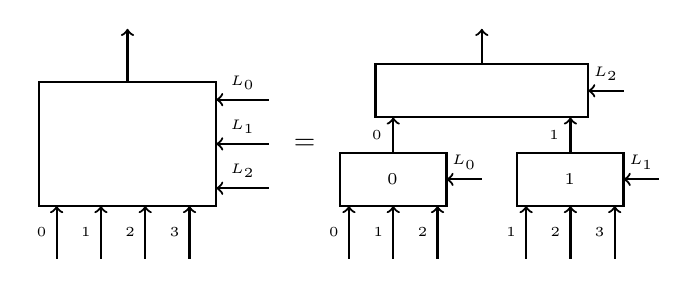
\begin{tikzpicture}[scale=0.45, yscale=1, thick] % , baseline = -3.5pt


\draw (-1,1) rectangle (4, 4.5);
\node[anchor=center] (text) at (1.5,2.75) {\small $\bencodingof{\lneuron}$};
\draw[->] (1.5,4.5)--(1.5,6) node[midway,right] {\tiny $\catvariableof{\lneuron}$}; 

\draw[<-] (4,4)--(5.5,4) node[midway,above] {\tiny $\fselectionvariable_{0}$}; 
\draw[<-] (4,2.75)--(5.5,2.75) node[midway,above] {\tiny $\fselectionvariable_{1}$}; 
\draw[<-] (4,1.5)--(5.5,1.5) node[midway,above] {\tiny $\fselectionvariable_{2}$}; 

\draw[<-] (-0.5,1)--(-0.5,-0.5) node[midway,left] {\tiny $\catvariableof{0}$}; 
\draw[<-] (0.75,1)--(0.75,-0.5) node[midway,left] {\tiny $\catvariableof{1}$}; 
\draw[<-] (2,1)--(2,-0.5) node[midway,left] {\tiny $\catvariableof{2}$}; 
\draw[<-] (3.25,1)--(3.25,-0.5) node[midway,left] {\tiny $\catvariableof{3}$}; 


\node[anchor=center] (text) at (6.5,2.75) {${=}$};


\draw (7.5,1) rectangle (10.5,2.5);
\node[anchor=center] (text) at (9,1.75) {\small $\bencodingof{\vselectionsymbol_0}$};
\draw[->] (9,2.5)--(9,3.5) node[midway,left] {\tiny $\catvariableof{\vselectionsymbol_0}$}; 

\draw[<-] (7.75,1)--(7.75,-0.5) node[midway,left] {\tiny $\catvariableof{0}$}; 
\draw[<-] (9,1)--(9,-0.5) node[midway,left] {\tiny $\catvariableof{1}$}; 
\draw[<-] (10.25,1)--(10.25,-0.5) node[midway,left] {\tiny $\catvariableof{2}$}; 
\draw[<-] (10.5,1.75)--(11.5,1.75) node[midway,above] {\tiny $\fselectionvariable_{0}$}; 

\draw (12.5,1) rectangle (15.5,2.5);
\node[anchor=center] (text) at (14,1.75) {\small $\bencodingof{\vselectionsymbol_1}$};
\draw[->] (14,2.5)--(14,3.5) node[midway,left] {\tiny $\catvariableof{\vselectionsymbol_1}$}; 

\draw[<-] (12.75,1)--(12.75,-0.5) node[midway,left] {\tiny $\catvariableof{1}$}; 
\draw[<-] (14,1)--(14,-0.5) node[midway,left] {\tiny $\catvariableof{2}$}; 
\draw[<-] (15.25,1)--(15.25,-0.5) node[midway,left] {\tiny $\catvariableof{3}$}; 
\draw[<-] (15.5,1.75)--(16.5,1.75) node[midway,above] {\tiny $\fselectionvariable_{1}$}; 

\draw (8.5,5) rectangle (14.5,3.5);
\node[anchor=center] (text) at (11.5,4.25) {\small $\bencodingof{\cselectionsymbol}$};
\draw[->] (11.5,5)--(11.5,6) node[midway,left] {\tiny $\catvariableof{\lneuron}$}; 
\draw[<-] (14.5,4.25)--(15.5,4.25) node[midway,above] {\tiny $\fselectionvariable_{2}$}; 

\end{tikzpicture}
\end{center}	
Where the variable selector cores $\bencodingof{\vselectionsymbol_0}$ and $\bencodingof{\vselectionsymbol_1}$ can be further decomposed into leg cores.
\end{frame}


\begin{frame}{Architectures}

Architectures are collections of neurons 
\begin{align*}
	\larchitecture = \{ \lneuron_0, \ldots , \lneuron_{n-1} \}
\end{align*}
which can depend on each other, i.e. a neuron can take another neuron as argument.

\medskip

We require \emph{acyclicity} of the possible dependencies 
\begin{itemize}
	\item for well-definedness of the resulting formulas (avoid circular dependencies)
	\item resulting in a feed-forward architecture of neurons based on the dependency order
\end{itemize}

\medskip

In this way, we can parametrize formulas with arbitrary complexity.

\end{frame}



\section{Architecture in Script Language}

\begin{frame}{Architecture specification in \tnreason}

We extend the nested lists encoding $\sencodingof{\exformula}$ defined for propositional formulas $\exformula$ to also encode 
\begin{itemize}
	\item Logical neurons $\lneuron$
	\item Formula selecting maps $\larchitecture$
\end{itemize}

Strategy: \emph{Choices captured in further nested lists}
\begin{itemize}
	\item Replace connectives by list of candidate connectives
	\item Replace direct subformula specifications by lists of variables (e.g. atomic variables or other neurons)
\end{itemize}

\end{frame}



\begin{frame}{Example: Wet street}

	Following the wet street example, we can define a neuron by
	\begin{centeredscript}
		$\sencodingof{\lneuron}$ = [[\stringof{imp},\stringof{eq}],[\stringof{Wet},\stringof{Sprinkler}],[\stringof{Street}]] 
	\end{centeredscript}
	from which the formulas 
	\begin{centeredscript}
		[\stringof{imp}, \stringof{Wet}, \stringof{Street}] \\
		\hspace{1cm} [\stringof{eq}, \stringof{Wet}, \stringof{Street}] \\
		\hspace{1cm}[\stringof{imp}, \stringof{Sprinkler}, \stringof{Street}] \\
		\hspace{1cm}[\stringof{eq}, \stringof{Sprinkler}, \stringof{Street}]		
	\end{centeredscript}
	can be chosen.
	Combining this neuron with further neurons, e.g. by the architecture
	\begin{centeredscript}
		$\sencodingof{\larchitecture}$ = \{ \stringof{neur1}: [[\stringof{imp},\stringof{eq}],[\stringof{neur2}],[\stringof{Street}]] , \\
		\hspace{1.8cm}\stringof{neur2}: [[\stringof{lnot},\stringof{id}],[\stringof{Wet},\stringof{Sprinkler}]] \}
	\end{centeredscript}
	the expressitivity increases.
	In this case, the further neuron provides the flexibility of the first atoms to be replaced by its negation.	

\end{frame}



\section{Optimization}



\begin{frame}{Optimization of the Likelihood}

Having a probability tensor $\probtensor$ as a current model, we want to find $\exformulain$ solving
	\[ \argmax_{\exformulain} \max_{\weight\in\rr} \lossof{\probtensor+\weight\cdot\exformula}  \, . \]

\begin{block}{Intractability of direct optimization}
	The likelihood involves partition functions and is not linear in $\exformula$.
	Therefore we cannot make use of the tensor network representation of $\fselectionmap$.
\end{block}

\end{frame}


\begin{frame}{Gradient Ascent Approach}


Extending a distribution $\probtensor$ by $\exformulain$ we have
\begin{align*}
	\frac{\partial}{\partial \weight} \lossof{\probtensor+\weight\cdot\exformula} |_{\weight=0}
	& = \expectationofwrt{\exformula}{\empdistribution} - \expectationofwrt{\exformula}{\probtensor} \\
	& = \contractionof{\{\empdistribution, \exformula\}}{\varnothing}
	 - \contractionof{\{\probtensor, \exformula\}}{\varnothing}
\end{align*}

We notice, that the partial derivative is linear in $\exformula$ and therefore, that we can express the gradient for all $\exformulain$ leaving the selection variable open
\begin{align*}
	\frac{\partial}{\partial \weight} \lossof{\probtensor+\sum_{\selindexin}\weightof{\exformula_{\selindex}}\cdot\exformula_{\selindex}} \Big|_{\weight=0}
	& = \contractionof{\empdistribution, \exformula}{\selinputvariable} - \contractionof{\probtensor, \exformula}{\selinputvariable} \, .
\end{align*}

\end{frame}



\begin{frame}{Gradient Ascent Approach}

\begin{block}{Likelihood gradient ascent}
	The problem of likelihood gradient ascent is solved by
	\begin{align*}
		\argmax_{\selindexin} \contractionof{\empdistribution, \exformula}{\selinputvariable} - \contractionof{\probtensor, \exformula}{\selinputvariable}
	\end{align*}
\end{block}

This is the search for the maximal coordinate of a tensor in a network representation.

\end{frame}


%\begin{frame}{Maximum likelihood estimation \\
%of Formula Selecting Neurons}
%
%Objectives $O$ are Tensor Networks 
%\begin{itemize}
%	\item representing \emph{probability distributions to be sampled}
%	\item representing (gradients of) \emph{log-likelihood given data} %(based on the Datacores $\datacoreof{\atomenumerator}$)
%%	\item differing in whether we differentiate and take the partition function into consideration
%\end{itemize}
%
%\begin{block}{Formalization: Max Coordinate Problem}
%	Having a Tensor Network and a subset of legs indexed by $\selindices$ solve
%		\[ \mathrm{argmax}_{\selindices} = \braket{O,\bencodingof{\exformula_{\selindices}}} \left(=\contractionof{\{
%		O,\bencodingof{\exformula_{\selindices}},\onehotmapof{\selindices}
%		\}}{\varnothing}\right)
%		 \, . \]
%\end{block}
%
%Solution algorithms:
%\begin{itemize}
%	\item Alternating optimization (e.g. Least Squares) of parameter cores in a decomposition format
%	\item Markov Chain Monte Carlo (e.g. Gibbs Sampling) 
%\end{itemize}
%
%
%\end{frame}




\begin{frame}{Algorithmic Efficiency}

%\begin{block}{Reasoning by tensor network contractions}
%	Reasoning workload is performed by (local/global) tensor network contractions.
%	How can we execute them in computational efficient ways? 
%\end{block}

Targeting space consumption: \emph{Tensor Network Decomposition}
\begin{itemize}
	\item Avoid the creation of high-dimensional tensors
	\item {Markov Logic Networks stored in local cores}
\end{itemize}

Targeting runtimes: \emph{Dynamic Programming}
\begin{itemize}
	\item Avoid the repetition of local contractions
	\item {Formula Selecting Architectures evaluate exponentially many formulas batchwise}
\end{itemize}

\begin{block}{Application in Inductive Logic Programming}
	Formula Selecting Architectures make use of the redundancies of propositional logics and provide a way to operate in large sets of formulas.
\end{block}

\end{frame}





\begin{frame}{Neuro-Symbolic AI for DATEV}

\begin{center}
	DATEV is an abbrevation of data processing \\ (in german: \emph{DATE}n-\emph{V}erarbeitung)
\end{center}
	\medskip

	
	\begin{columns}
		
		\column{0.5 \linewidth}
		\textbf{Traditional Approach} 
		\begin{itemize}
			\item Logic hard-coded in programs
			\item Processing by coded formulas 
			\item User has full control
		\end{itemize}

		
		\column{0.5 \linewidth}
		\textbf{Data-driven Approach} 
		\begin{itemize}
			\item Learn logic from data 
			\item Uncertainty tolerant processing
			\item User desires control
		\end{itemize}
		
	\end{columns}
	
	\medskip
	
	\begin{block}{Advantages of Neuro-Symbolic Methods}
		\begin{itemize}
			\item Exploit expert knowledge when learning models or designing them declaratively 
			\item Maintain control through intrinsic model interpretability
			\item Minimize user interaction by uncertainty assessments
		\end{itemize}
%		Intrinsic explainability of models is of central importance (more than in other companies).
%		Can we provide efficient methods based on neuro-symbolic architectures?
	\end{block}
	
\end{frame}










\end{document}

